\section{Method}

\begin{frame}
	\frametitle{Contributions}
	
	\Large
	
	\vspace{0.8cm}
	
	We present an automated approach for classifying Alzheimer's disease patients from MRI brain scans.
	
	\begin{enumerate}
		\item key points extracted with a \textbf{recent} feature extraction technique, called ORB
			  \cite{Rublee11}
		\item final set of features obtained by \textbf{defining} two \textbf{new} metrics:
			  \textbf{spatial position} of extracted key points and \textbf{their distribution} around
			  the patient's brain
		\item \textbf{fast} and \textbf{reliable} approach for a straightforward deploy in clinical
			  applications
	\end{enumerate}
	
	\vspace{0.58cm}
	
	\tiny
	
	\cite{Rublee11} E. Rublee \emph{et al.}, ``ORB: an efficient alternative to SIFT or SURF'',
	International Conference on Computer Vision, 2011
\end{frame}

\begin{frame}
	\frametitle{Methodology}
	
	\Large
	
	\vspace{0.7cm}
	
	We focus on extracting features which are \textbf{key points} found in the image. In particular, we
	choose as features a set of key points from the MRI scan \textbf{computed} with the ORB feature
	extractor, and we \textbf{associate} to them their \textbf{spatial position} and
	\textbf{distribution} around the patient's brain.
	
	\begin{center}
		\begin{tikzpicture}
			\node at (-5.5,0) [draw=white,ultra thick,inner sep=0pt]
			{
				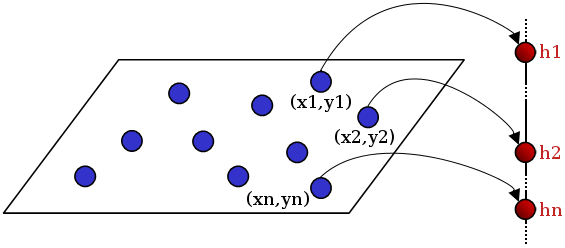
\includegraphics[height=2.5cm]{Figures/CantorHash}
			};
			\node at (0,0) [draw=white,ultra thick,inner sep=0pt]
			{
				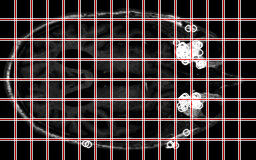
\includegraphics[height=2.5cm]{Figures/Histograms}
			};
		\end{tikzpicture}
	\end{center}
\end{frame}

\begin{frame}
	\frametitle{Methodology}
	\framesubtitle{Key point features}
	
	\Large
	
	\vspace{0.7cm}
	
	Many different approaches have been proposed for feature extraction. We focus on a
	\textbf{computationally-efficient} technique - called ORB - which is based on a FAST key point
	detector. It provides \textbf{good matching}, \textbf{slighlty} affected by image noise and
	\textbf{real-time} performance.
	
	\vspace{0.1cm}
	
	\begin{center}
		\begin{tikzpicture}
			\node at (-2.6,0) [draw=red,ultra thick,inner sep=0pt]
			{
				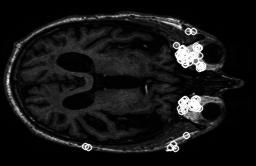
\includegraphics[height=2.5cm]{Figures/OrbKeypoint}
			};
			\node at (0,0) [draw=red,ultra thick,inner sep=0pt]
			{
				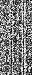
\includegraphics[height=2.5cm]{Figures/OrbDescriptor}
			};
		\end{tikzpicture}
	\end{center}
\end{frame}

\begin{frame}
	\frametitle{Methodology}
	\framesubtitle{Key point features}
	
	\Large
	
	\begin{columns}[T]
		\column{0.35\textwidth}
		
		\begin{center}
			\begin{tikzpicture}
				\node at (0,0) [draw=red,ultra thick,inner sep=0pt]
				{
					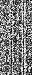
\includegraphics[height=3.5cm]{Figures/OrbDescriptor}
				};
			\end{tikzpicture}
		\end{center}
		
		\column{0.58\textwidth}
		
		\vspace{0.65cm}
		
		The feature descriptor of each key point is a \textbf{32-vector} of the pixel
		\textbf{intensity}. The image is described by a $ k \times 32 $ matrix, where $ k $ represents
		the number of key points found in the image.
		
		\column{0.05\textwidth}
	\end{columns}
\end{frame}
